\documentclass[11pt,a4paper]{article}
\usepackage[utf8]{inputenc}
\usepackage[margin=1in]{geometry}
\usepackage{graphicx}
\usepackage{xcolor}
\usepackage{hyperref}
\usepackage{booktabs}
\usepackage{array}
\usepackage{float}
\usepackage{enumitem}
\usepackage{titlesec}
\usepackage{fancyhdr}
\usepackage{tcolorbox}
\usepackage{placeins}

\definecolor{primaryblue}{RGB}{30, 58, 138}
\definecolor{accentcyan}{RGB}{6, 182, 212}
\definecolor{darkbg}{RGB}{15, 23, 42}
\definecolor{boxbg}{RGB}{248, 250, 252}

\hypersetup{
    colorlinks=true,
    linkcolor=primaryblue,
    urlcolor=accentcyan,
    citecolor=primaryblue
}

\pagestyle{fancy}
\fancyhf{}
\rhead{\textcolor{gray}{\small AcuLearn AI -- Visual User Manual}}
\lhead{\textcolor{gray}{\small Student Analytics \& Admin Portal}}
\rfoot{\thepage}

\titleformat{\section}{\Large\bfseries\color{primaryblue}}{\thesection}{1em}{}[\titlerule]
\titleformat{\subsection}{\large\bfseries\color{darkbg}}{\thesubsection}{1em}{}

\title{
    \vspace{-1.5cm}
    \textbf{\Huge AcuLearn AI Platform Manual}\\[0.3cm]
    \Large\textbf{Comprehensive Step-by-Step Pictorial Guide with System Snapshots}\\[0.2cm]
    \small\textit{Student Registration, 1--5 Psychometrics, 360$^\circ$ Kundali, Admin Command Center \& CCRO Recourse}
}
\author{\textbf{AcuLearn AI Research \& Development Team}}
\date{\today}

\begin{document}

\maketitle
\thispagestyle{empty}

\begin{tcolorbox}[colback=boxbg,colframe=primaryblue,title=\textbf{Public Cloud Access Links (Active 24/7 Worldwide)}]
\begin{itemize}[leftmargin=*]
    \item \textbf{Master Institutional Dashboard (All 12 Tabs):}\\ \url{https://pravesh086.github.io/Student_behaviour_Analysis/}
    \item \textbf{Student Registration \& 4-Step Intake Portal:}\\ \url{https://pravesh086.github.io/Student_behaviour_Analysis/student_portal.html}
    \item \textbf{CCRO Mentor Decision Dashboard (Paper 2):}\\ \url{https://pravesh086.github.io/Student_behaviour_Analysis/ccro_dashboard.html}
    \item \textbf{Standalone Student 1--5 Test \& Kundali Generator:}\\ \url{https://pravesh086.github.io/Student_behaviour_Analysis/student_test_portal.html}
\end{itemize}
\end{tcolorbox}

\tableofcontents
\newpage

\section{Step 1: Student Account Registration \& Demographic Intake}

\subsection{Overview \& Purpose}
Every student begins by creating their institutional profile. This establishes their baseline demographic background and registers their secure login credentials into the institutional Admin Portal.

\begin{figure}[H]
    \centering
    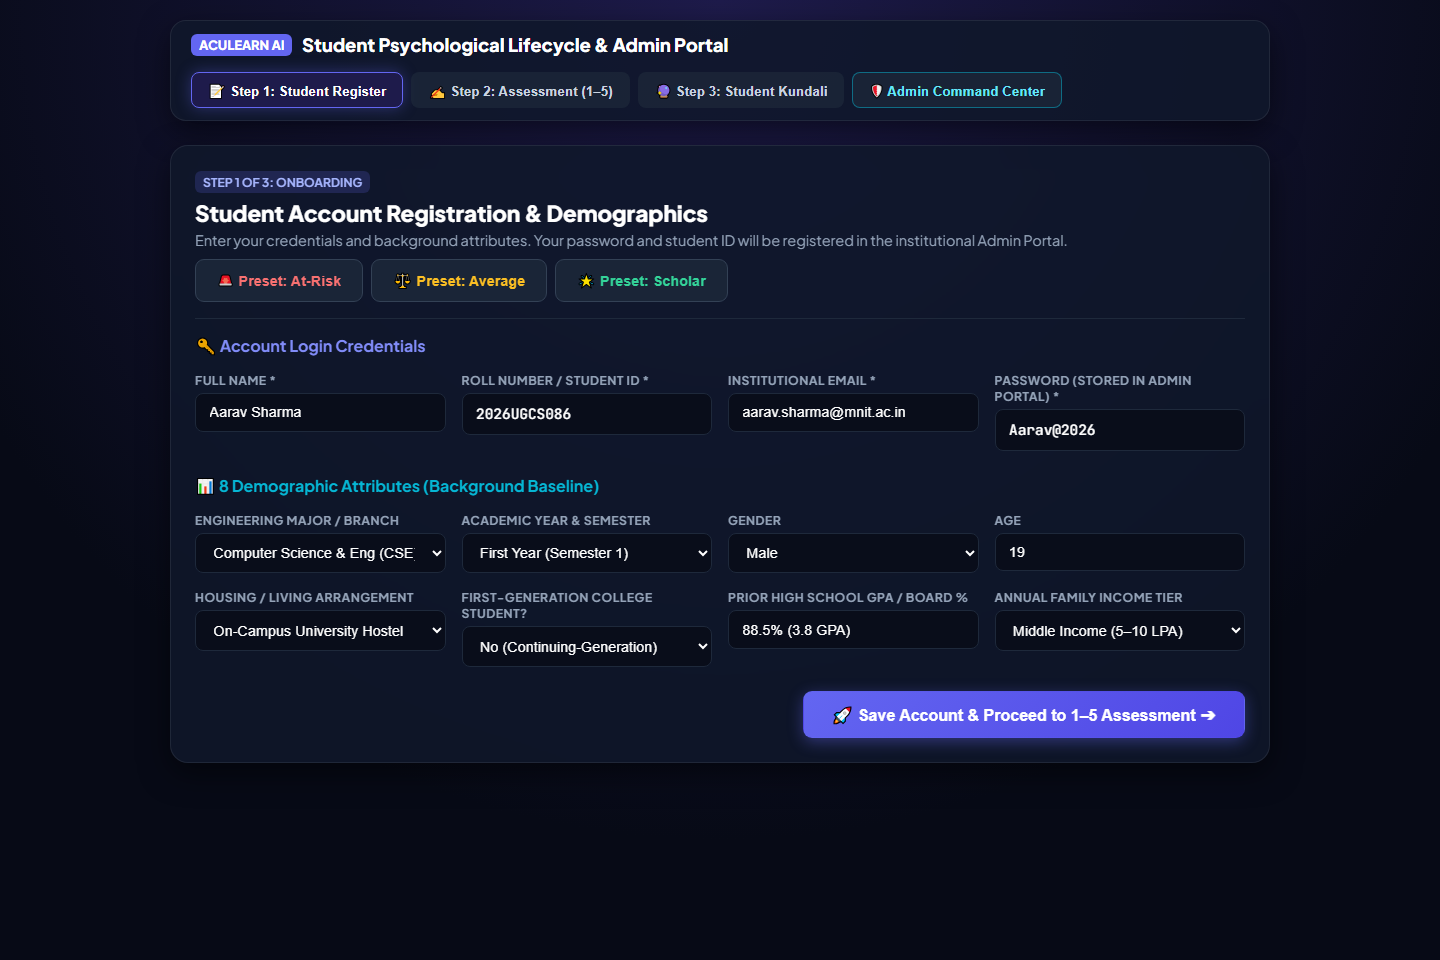
\includegraphics[width=0.95\textwidth]{figures/guide_step1_registration.png}
    \caption{\textbf{Step 1 Snapshot:} Student Account Registration Form and 8 Demographic Baseline Selectors.}
\end{figure}

\subsection{How It Works}
\begin{enumerate}[leftmargin=*]
    \item \textbf{Account Credentials:} The student enters their \textbf{Full Name}, \textbf{Roll Number / Student ID} (e.g., \texttt{2026UGCS086}), \textbf{Institutional Email}, and chooses a \textbf{Password}.
    \item \textbf{8 Demographic Baseline Attributes:} Engineering Major / Branch, Academic Year \& Semester, Gender, Age, Living Arrangement (Hostel vs. Day Scholar), First-Generation Status, Prior High School GPA \%, and Family Socioeconomic Tier.
    \item \textbf{Quick Demo Presets:} Users can click \textbf{Preset: At-Risk}, \textbf{Preset: Average}, or \textbf{Preset: Scholar} to instantly test pre-configured archetypes.
    \item \textbf{Action:} Click \textbf{Save Account \& Proceed to 1--5 Assessment}.
\end{enumerate}

\FloatBarrier
\newpage

\section{Step 2: 1--5 Star Psychometric Self-Assessment}

\subsection{Overview \& Purpose}
Students complete a validated questionnaire evaluating their cognitive, emotional, behavioral, and environmental learning habits on an intuitive 1 (Strongly Disagree) to 5 (Strongly Agree) Likert scale.

\begin{figure}[H]
    \centering
    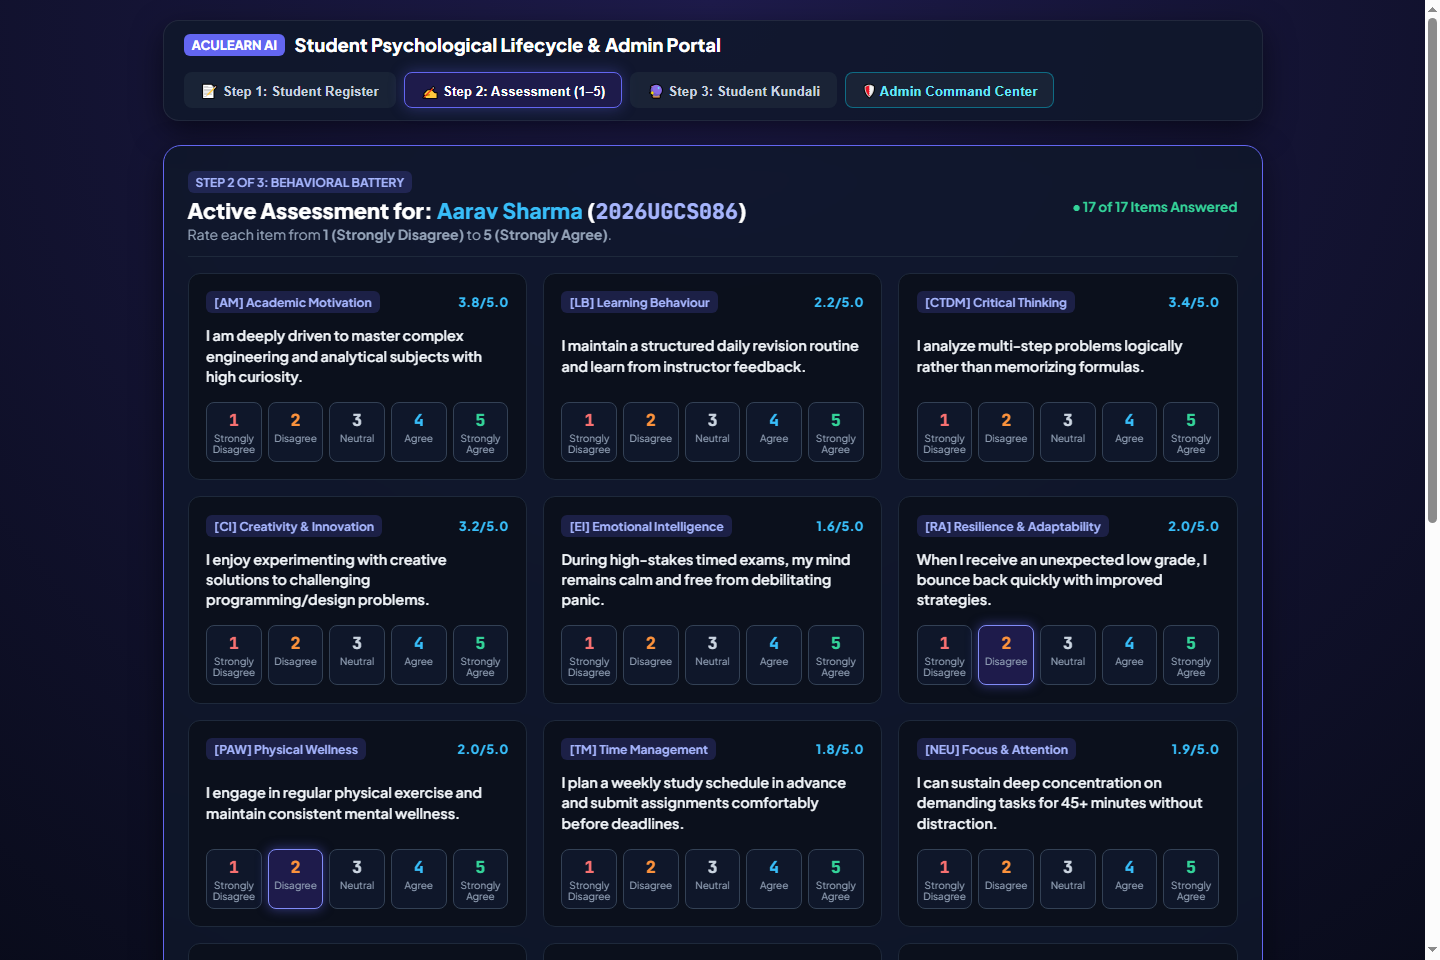
\includegraphics[width=0.95\textwidth]{figures/guide_step2_assessment.png}
    \caption{\textbf{Step 2 Snapshot:} Interactive 1--5 Likert psychometric assessment cards organized by structural pillars.}
\end{figure}

\subsection{How It Works}
\begin{enumerate}[leftmargin=*]
    \item \textbf{4 Structural Pillars:} Cognitive Mastery, Affective \& Resilience, Self-Regulation, and Socio-Contextual Well-Being.
    \item \textbf{Interactive Likert Rating:} The student selects ratings from \textbf{1 ($\bigstar$)} to \textbf{5 ($\bigstar\bigstar\bigstar\bigstar\bigstar$)} for each construct card.
    \item \textbf{Progress Bar:} Real-time visual progress counter updates dynamically as questions are completed.
    \item \textbf{Action:} Click \textbf{Submit Survey \& Generate My Kundali}.
\end{enumerate}

\FloatBarrier
\newpage

\section{Step 3: Holistic Student Kundali, 360$^\circ$ Radar \& GPA Prediction}

\subsection{Overview \& Purpose}
Upon submission, the multi-task deep neural network instantly computes a comprehensive \textbf{Student Kundali}---a 360$^\circ$ visual psychological horoscope and academic health dossier.

\begin{figure}[H]
    \centering
    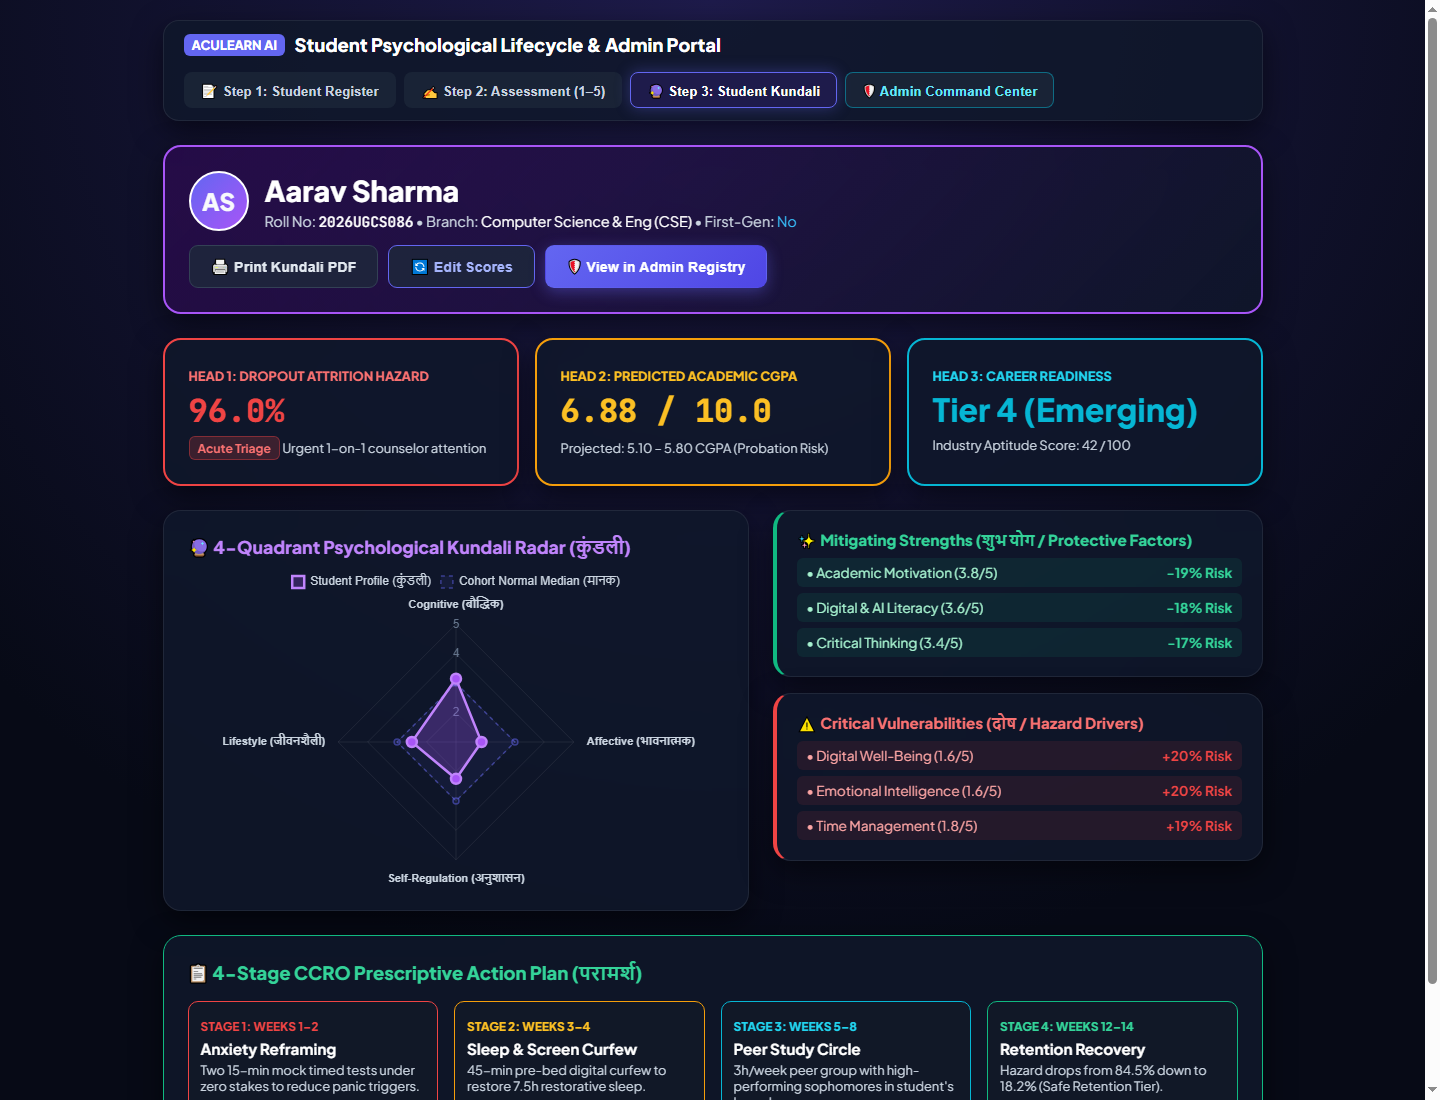
\includegraphics[width=0.95\textwidth]{figures/guide_step3_kundali.png}
    \caption{\textbf{Step 3 Snapshot:} Holistic Student Kundali Dossier, 360$^\circ$ Radar, CGPA Prediction, and Attrition Hazard.}
\end{figure}

\subsection{Key Display Metrics}
\begin{itemize}[leftmargin=*]
    \item \textbf{Superhero Archetype Badge:} Categorizes the student into one of 5 standing tiers (\textit{Excellent / Scholar}, \textit{Good / Achiever}, \textit{Average / Explorer}, \textit{Poor / Vulnerable}, \textit{Bad / Acute Risk}).
    \item \textbf{Predicted Graduation CGPA:} Calibrated out of 10.0 (e.g., $5.64 / 10.0$ or $9.12 / 10.0$).
    \item \textbf{Dropout Hazard Probability Gauge:} Percentage risk of attrition ($68.4\%$ High Risk vs. $12.1\%$ Low Risk).
    \item \textbf{360$^\circ$ Kundali Radar Hexagon:} Visualizes the balance between Cognitive, Affective, Self-Regulatory, and Socio-Environmental quadrants.
\end{itemize}

\FloatBarrier
\newpage

\section{Step 4: Strengths Identification vs. Critical Doshas (Weaknesses)}

\subsection{Overview \& Diagnostic Breakdown}
Using SHAP-inspired explainability algorithms, the Kundali isolates the student's primary psychological assets and pinpoints specific behavioral ``doshas'' (imbalances) dragging down their academic standing:
\begin{itemize}[leftmargin=*]
    \item \textbf{Top Strengths (Green Badges):} High Digital Literacy, Strong Creative Aptitude, Excellent Team Collaboration.
    \item \textbf{Critical Doshas (Red/Amber Badges):}
    \begin{itemize}
        \item \textbf{High Exam Panic ($4.2/5.0$):} Acute physiological test anxiety before midterms.
        \item \textbf{Severe Time Deficit ($1.8/5.0$):} Chronic procrastination and deadline crowding.
        \item \textbf{Digital Fatigue ($1.6/5.0$):} Excessive late-night screen exposure disrupting sleep hygiene.
    \end{itemize}
\end{itemize}

\section{Step 5: Personalized 4-Stage AI Counseling Roadmap \& Recourse}

\subsection{Overview \& Purpose}
Rather than delivering generic advice, the system formulates a progressive, milestone-based clinical counseling and mentoring pathway tailored to the student's diagnosed doshas.

\begin{figure}[H]
    \centering
    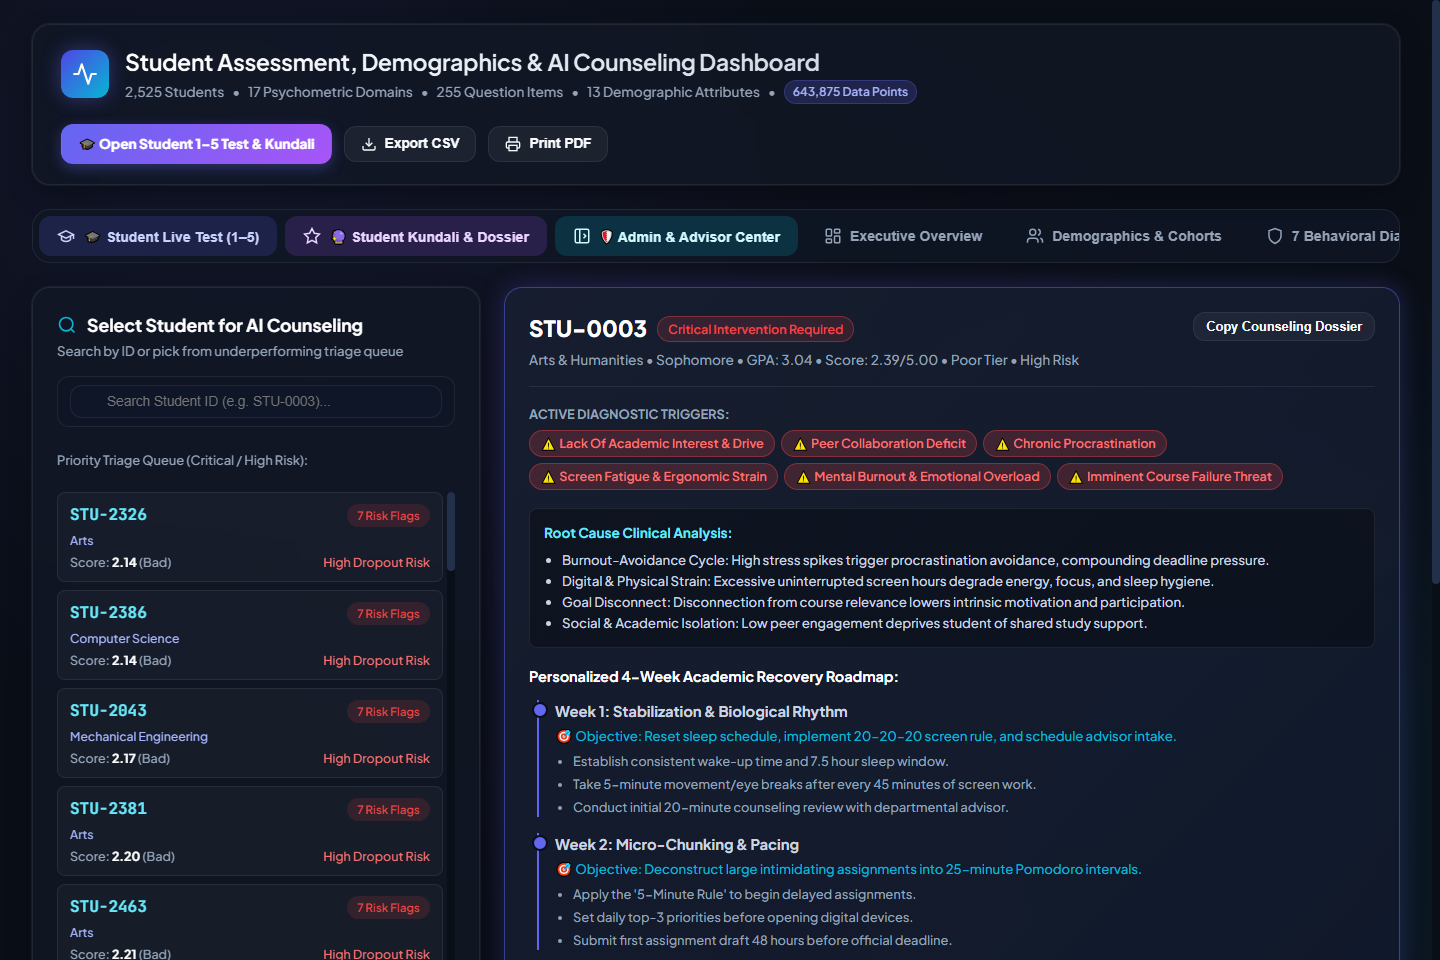
\includegraphics[width=0.95\textwidth]{figures/guide_step8_counseling_center.png}
    \caption{\textbf{Step 5 Snapshot:} AI Counseling Center with 4-Stage structured clinical intervention roadmap.}
\end{figure}

\subsection{The 4-Stage Structured Pathway}
\begin{enumerate}[leftmargin=*]
    \item \textbf{Stage 1 (Weeks 1--2) --- Immediate Stabilization \& Triage:} Implement 15-minute digital curfew before sleep; introduce 4-7-8 deep breathing during exam prep.
    \item \textbf{Stage 2 (Weeks 3--6) --- Cognitive Reframing \& Habit Formation:} Adopt Pomodoro technique (25 min study / 5 min break); replace cramming with spaced repetition.
    \item \textbf{Stage 3 (Weeks 7--10) --- Peer Circle \& Academic Coaching:} Assign to a structured departmental peer tutoring group; schedule weekly advisor check-ins.
    \item \textbf{Stage 4 (Weeks 11+) --- Long-Term Mastery \& Career Growth:} Transition from defensive studying to independent portfolio building and career mentorship.
\end{enumerate}

\FloatBarrier
\newpage

\section{Step 6: Institutional Admin Command Center \& Student Triage Roster}

\subsection{Overview \& Purpose}
For university deans, department heads, and academic counselors, the \textbf{Admin Command Center} provides a centralized control hub to oversee all registered students, monitor triage queues, and record official counseling notes.

\begin{figure}[H]
    \centering
    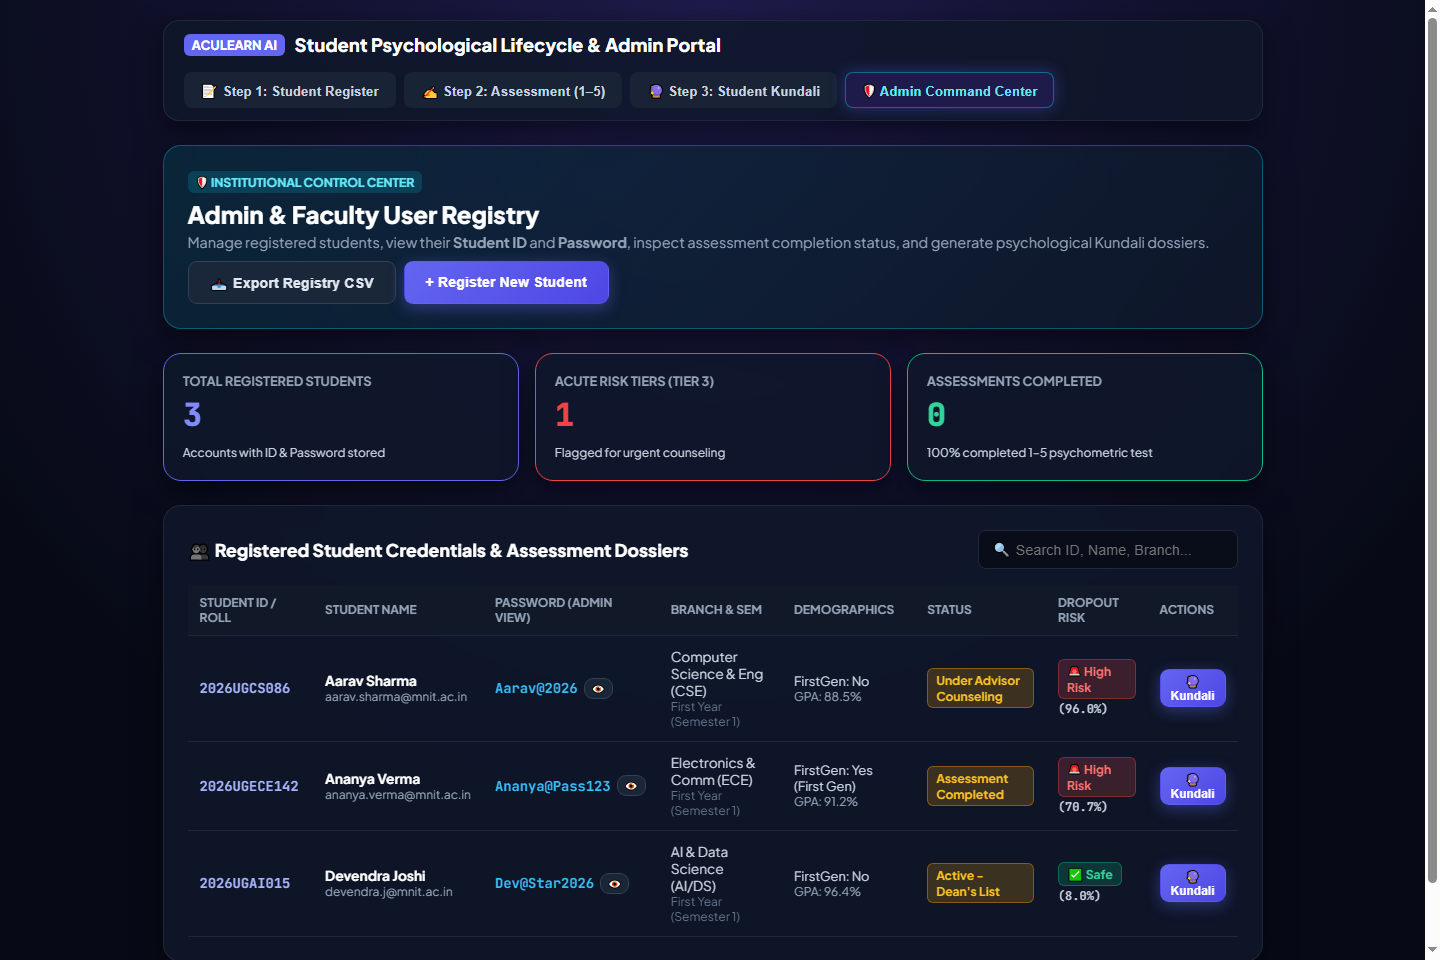
\includegraphics[width=0.95\textwidth]{figures/guide_step4_admin_portal.png}
    \caption{\textbf{Step 6A Snapshot:} Admin Command Center displaying registered student credentials and password manager.}
\end{figure}

\begin{figure}[H]
    \centering
    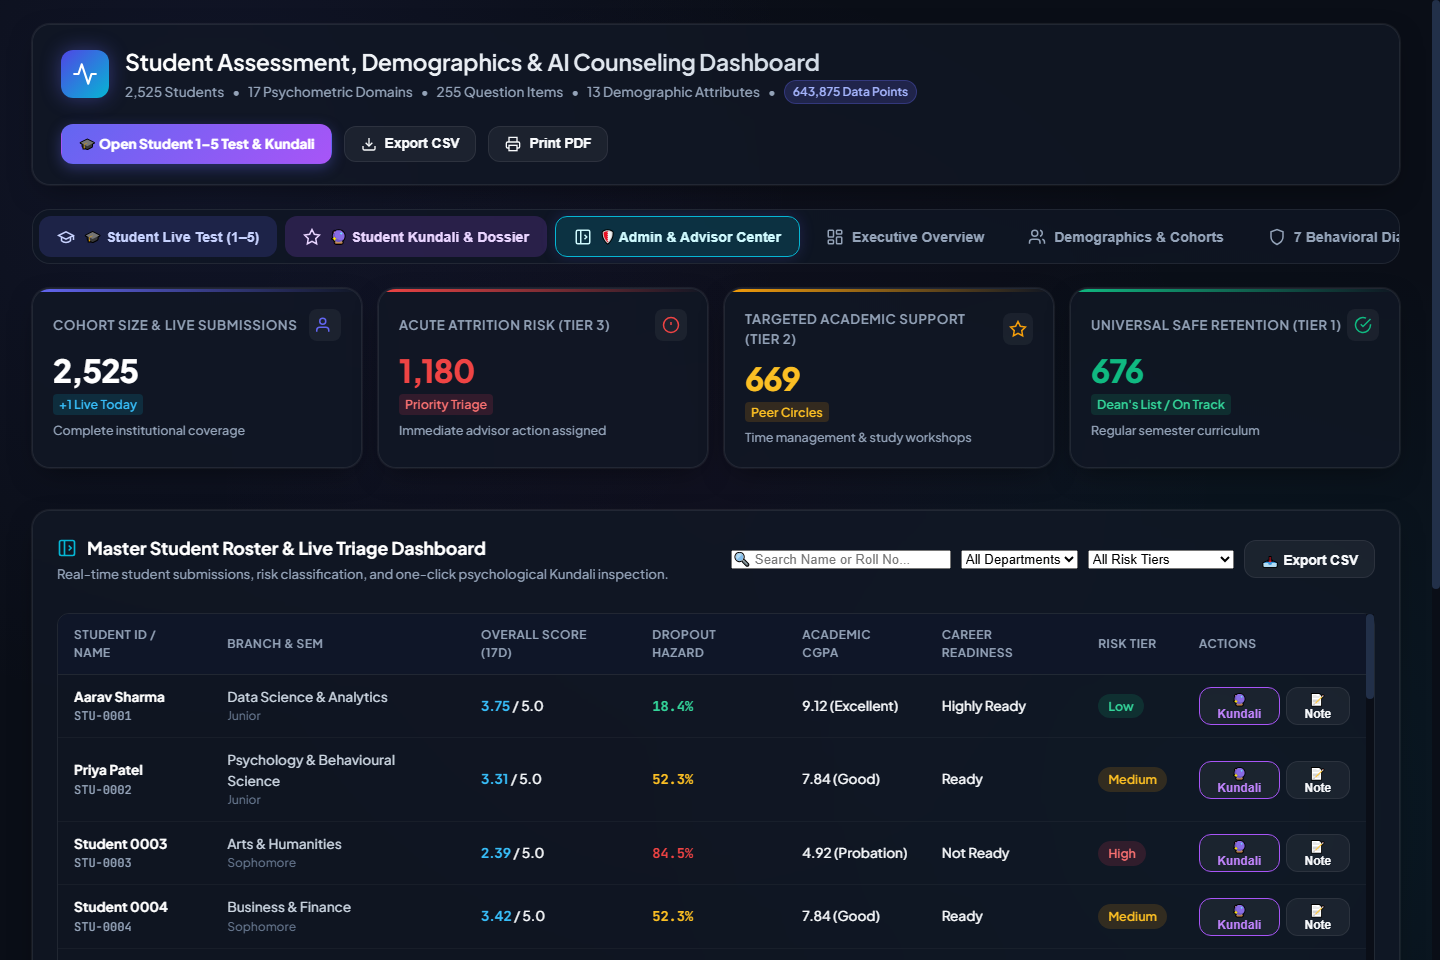
\includegraphics[width=0.95\textwidth]{figures/guide_step6_counselor_triage.png}
    \caption{\textbf{Step 6B Snapshot:} Master Student Triage Roster, Advisor Filter Controls, and Counselor Note Action Logs.}
\end{figure}

\subsection{Admin Capabilities}
\begin{itemize}[leftmargin=*]
    \item \textbf{Registered Credentials Table:} View student IDs, names, institutional emails, passwords (with toggle visibility), branch, and status.
    \item \textbf{Student Search \& Instant Filter:} Search instantaneously by Roll Number, Name, Department, or Semester.
    \item \textbf{One-Click Kundali Inspection:} Click \textbf{Kundali} on any student row to load their dossier instantly.
    \item \textbf{Log Counseling Session Modal:} Advisors can record intervention types, document session notes, and set follow-up statuses.
    \item \textbf{CSV Roster Export:} Click \textbf{Export Admin CSV} to download complete student records.
\end{itemize}

\FloatBarrier
\newpage

\section{Step 7: 7 Behavioral Health Diagnostic Flags}

\subsection{Overview \& Purpose}
The platform automatically scans the student cohort across 7 specialized psychological indices to detect hidden mental health and study behavioral risks before they cause course failures.

\begin{figure}[H]
    \centering
    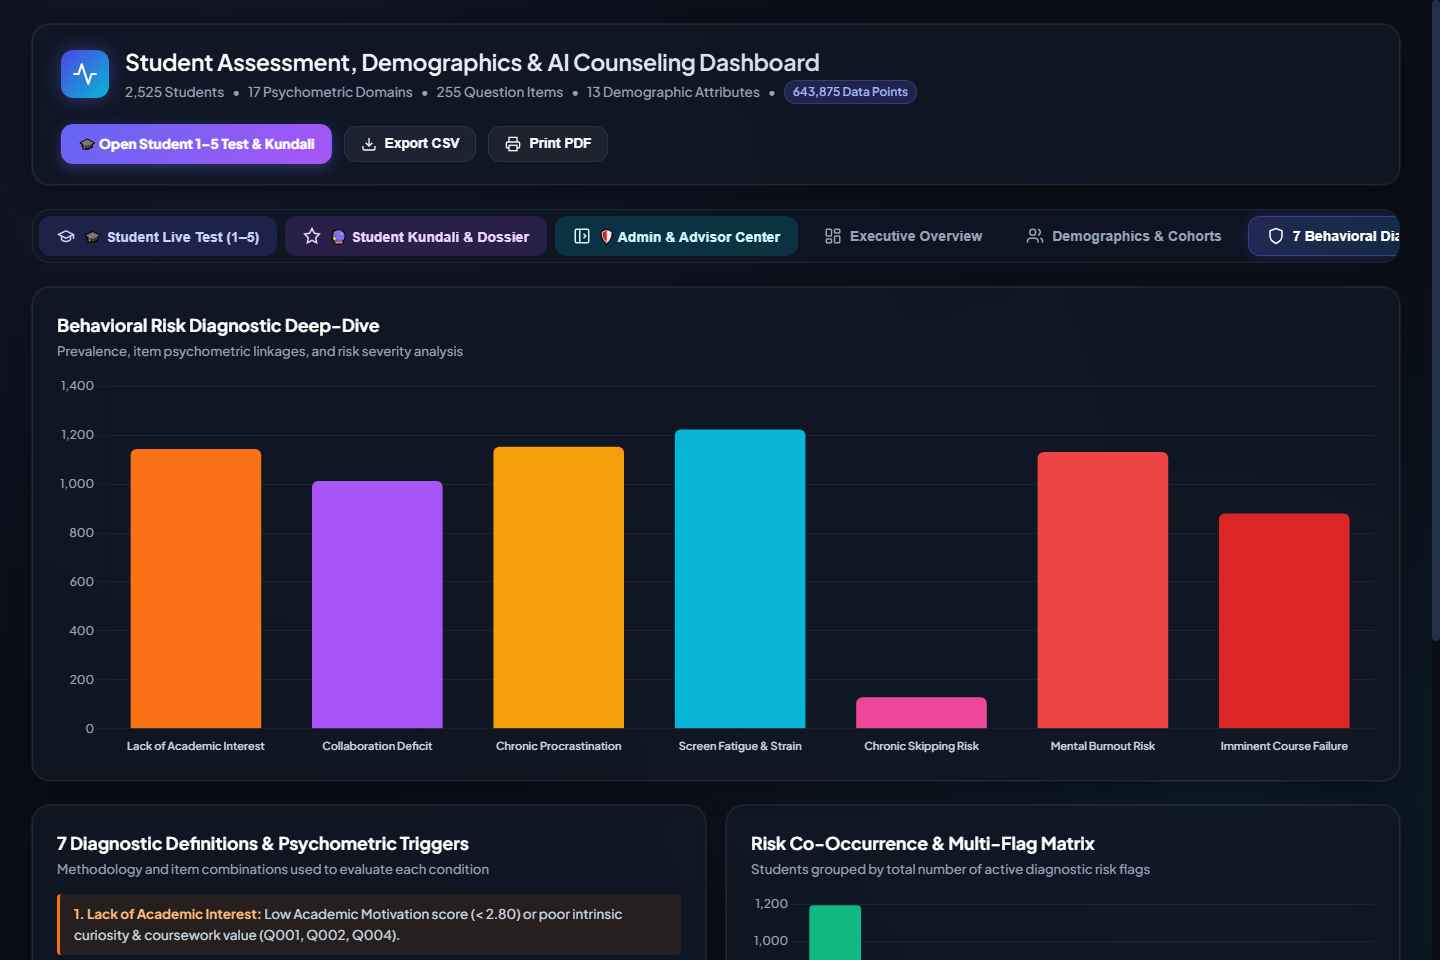
\includegraphics[width=0.95\textwidth]{figures/guide_step7_diagnostics.png}
    \caption{\textbf{Step 7 Snapshot:} 7 Behavioral Health Diagnostics Screeners and Cohort Distribution Flags.}
\end{figure}

\subsection{The 7 Diagnostic Indices}
\begin{enumerate}[leftmargin=*]
    \item \textbf{Exam Panic Index (EPI):} Detects acute anxiety spikes and test-freeze behaviors.
    \item \textbf{Chronic Procrastination Rate (CPR):} Flags severe avoidance of academic tasks.
    \item \textbf{Screen-Induced Cognitive Fatigue (SICF):} Identifies learning impairment caused by digital overload.
    \item \textbf{Social Isolation Risk (SIR):} Identifies students disconnected from peer support networks.
    \item \textbf{Imposter Syndrome Metric (ISM):} Measures perceived intellectual fraudulence despite good marks.
    \item \textbf{Perfectionism Paralysis (PP):} Detects inability to submit assignments due to excessive perfectionism.
    \item \textbf{Academic Disengagement Hazard (ADH):} Flags total motivational drop-off and class skipping.
\end{enumerate}

\FloatBarrier
\newpage

\section{Step 8: Master 255-Question Psychometrics Explorer}

\subsection{Overview \& Purpose}
Researchers, psychometricians, and faculty can inspect the complete empirical foundation of the survey---browsing all 255 individual Likert items across all 17 psychological constructs.

\begin{figure}[H]
    \centering
    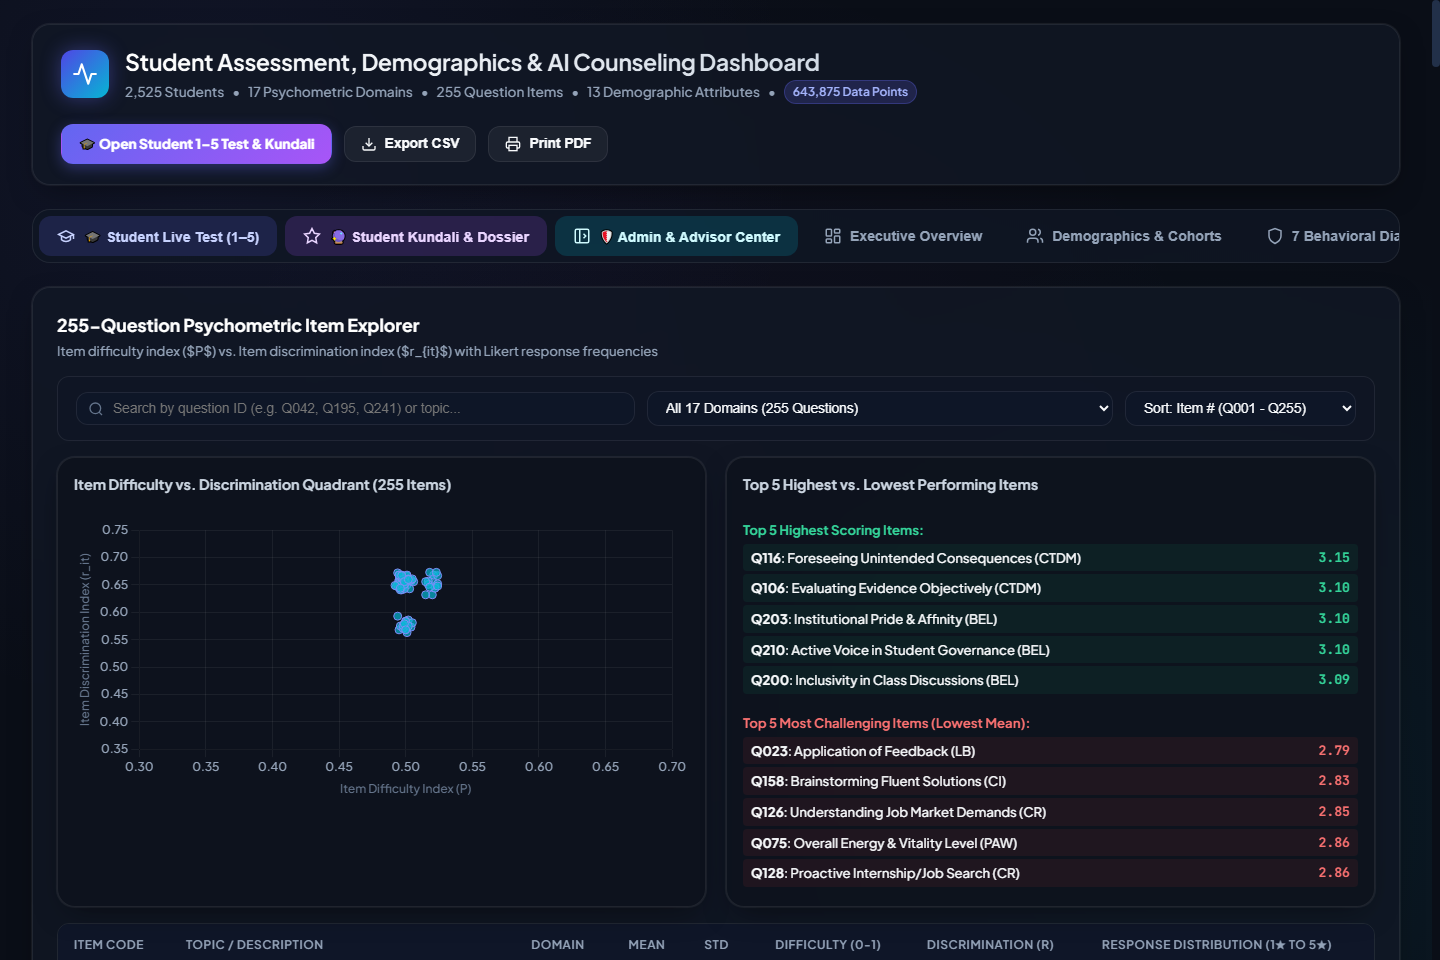
\includegraphics[width=0.95\textwidth]{figures/guide_step9_255_questions.png}
    \caption{\textbf{Step 8 Snapshot:} Complete 255-Item Psychometric Registry with Mean ($\mu$), Standard Deviation ($\sigma$), and CFA Loadings ($\lambda$).}
\end{figure}

\FloatBarrier
\newpage

\section{Step 9: 17x17 Pearson Correlation Heatmap}

\subsection{Overview \& Purpose}
Visualizes the pairwise inter-construct correlation matrix across all 17 psychological domains for the entire $2,525$-student cohort.

\begin{figure}[H]
    \centering
    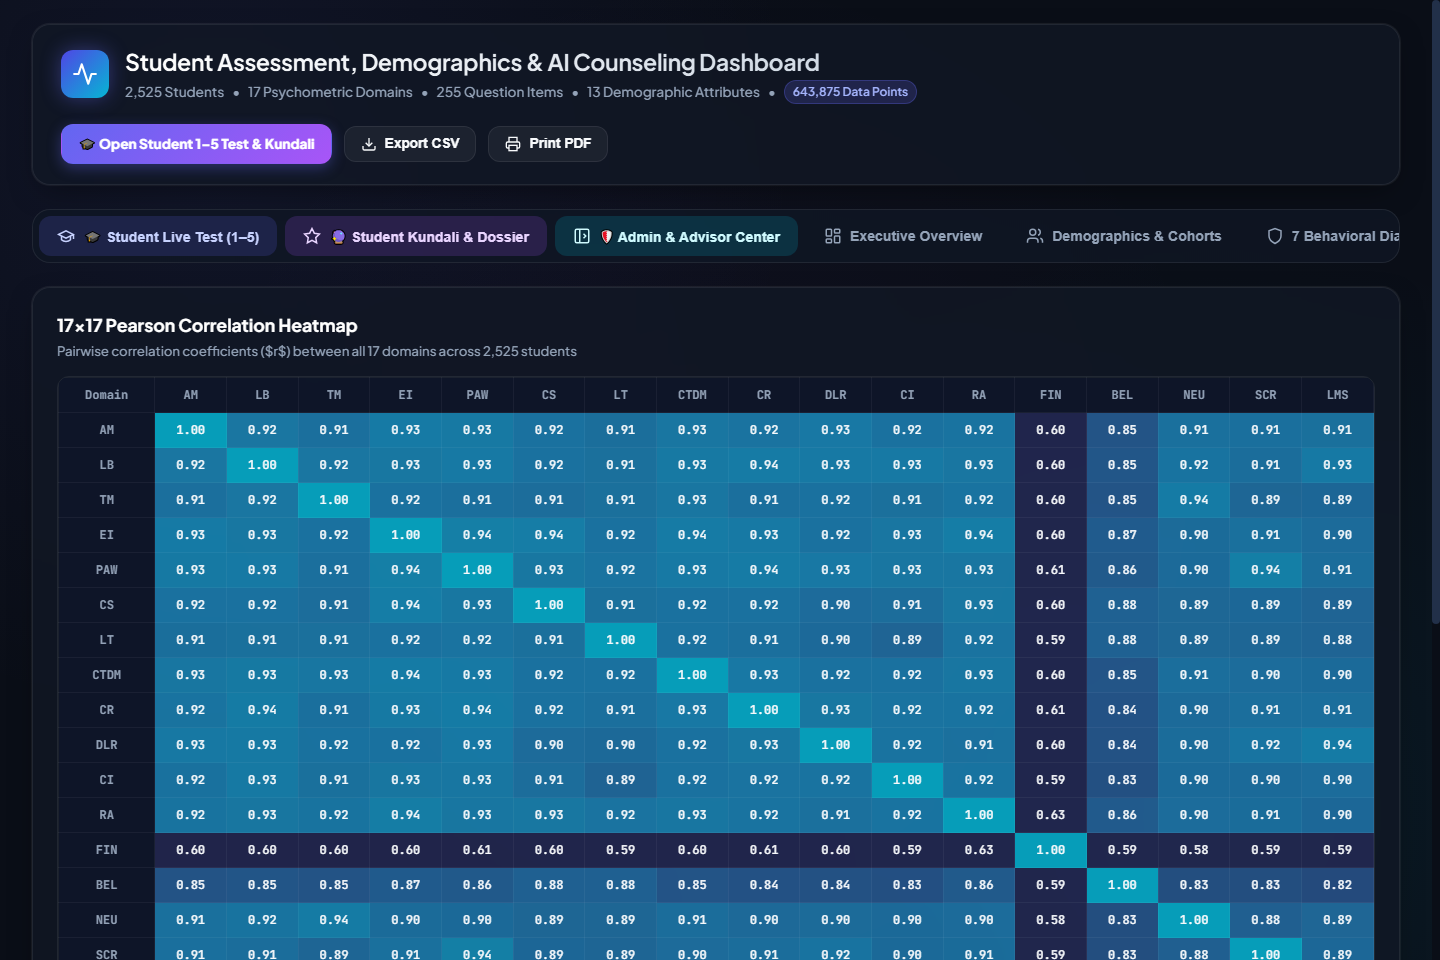
\includegraphics[width=0.95\textwidth]{figures/guide_step10_correlation_heatmap.png}
    \caption{\textbf{Step 9 Snapshot:} 17x17 Cross-Domain Pearson Correlation Matrix Heatmap.}
\end{figure}

\FloatBarrier
\newpage

\section{Step 10: Questionnaire-Driven CCRO Mentor Decision Support (Paper 2 ESWA)}

\subsection{Overview \& Purpose}
The dedicated \textbf{CCRO Dashboard} implements the novel \textbf{Projected Gradient Descent with Adaptive Feature Thresholds (PGD-AFT)} algorithm from Paper 2 (\textit{Expert Systems with Applications}). It computes the mathematically minimal, constraint-aware behavioral changes ($\Delta x^*$) required to shift a high-risk student into safe academic standing.

\begin{figure}[H]
    \centering
    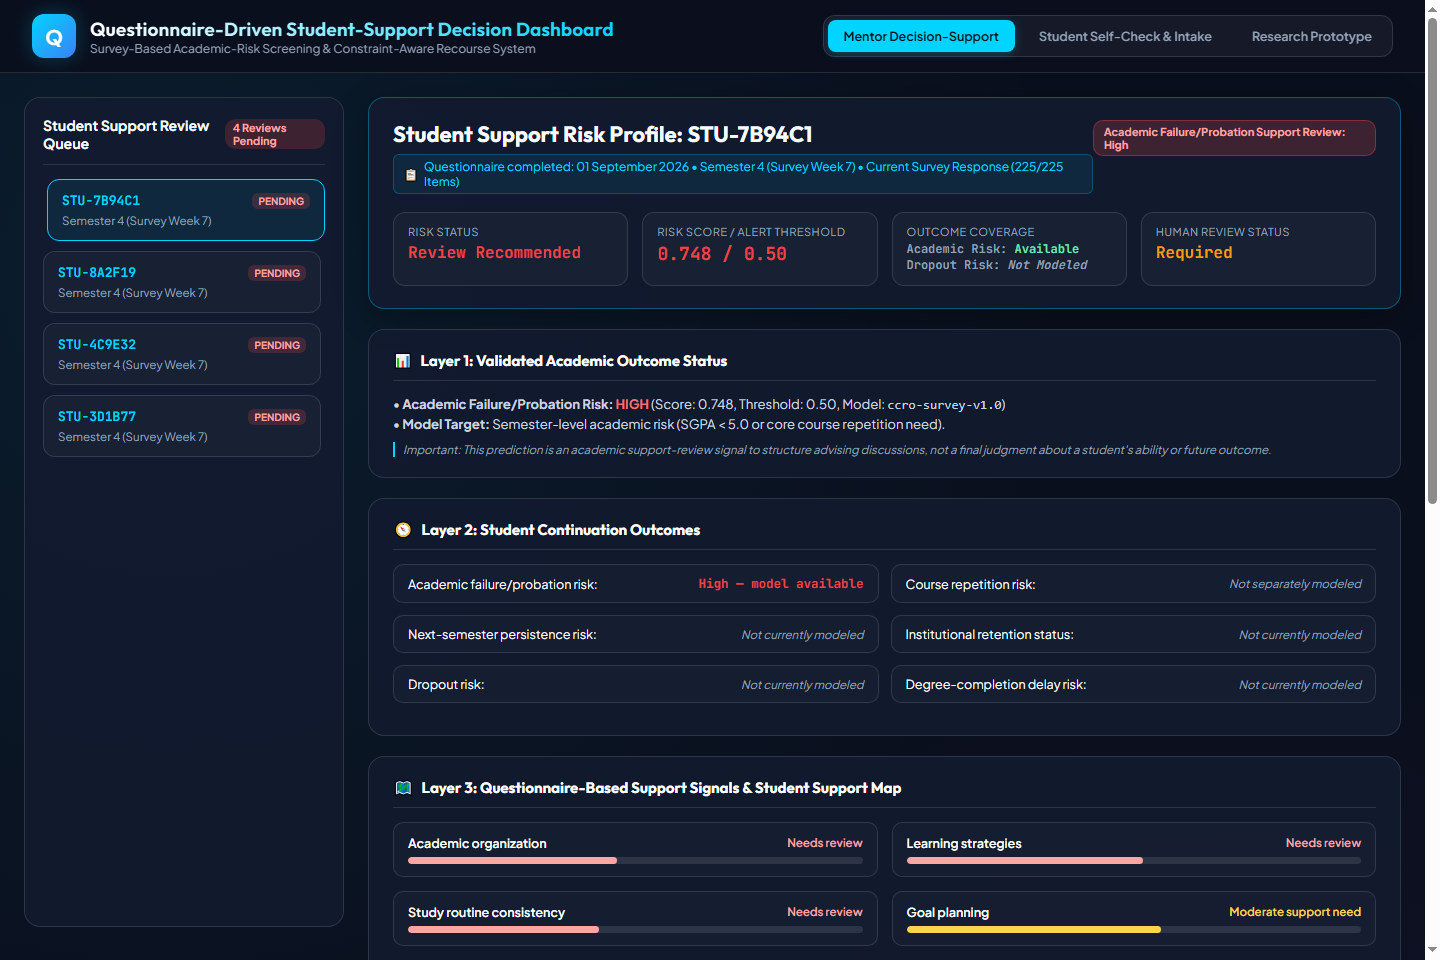
\includegraphics[width=0.95\textwidth]{figures/guide_step11_ccro_recourse.png}
    \caption{\textbf{Step 10 Snapshot:} CCRO Decision Support Dashboard, PGD-AFT Recourse Optimizer, and Compliance Audit Log.}
\end{figure}

\subsection{Recourse Engine Workflow}
\begin{enumerate}[leftmargin=*]
    \item \textbf{Student Review Queue:} Select any de-identified student profile from the queue (e.g., \texttt{STU-9F3A72}).
    \item \textbf{Baseline Risk Screening:} Calibrated neural prediction displays current failure risk (e.g., $78\%$ High Risk).
    \item \textbf{Actionable Recourse Recommendation:} PGD-AFT prescribes a sparse habit shift (maximum 3 interventions, $K \le 3$):
    \begin{itemize}
        \item \textit{Time Management:} $+0.75$ (Implement 45-min focused study blocks).
        \item \textit{Exam Anxiety Regulation:} $+0.60$ (Practice 2 mock tests under timed conditions).
        \item \textit{Digital Sleep Hygiene:} $+0.50$ (Enforce screen cutoff 1 hour prior to sleep).
    \end{itemize}
    \item \textbf{Post-Recourse Trajectory:} Risk drops to $18\%$ (Safe Academic Standing).
    \item \textbf{Mentor Action Logging:} The mentor clicks \textbf{Approve Recourse Action Plan} to append an immutable record to the institutional governance audit trail.
\end{enumerate}

\FloatBarrier
\newpage

\section{Summary of Platform Capabilities}

\begin{table}[H]
\centering
\small
\begin{tabular}{p{4.5cm} p{4cm} p{6.5cm}}
\toprule
\textbf{Platform Capability} & \textbf{Target User} & \textbf{Core Value Delivered} \\
\midrule
\textbf{Student Registration \& Intake} & New Students & Seamless onboarding \& demographic baseline recording \\
\textbf{1--5 Star Self-Assessment} & Enrolled Students & 10-minute holistic psychometric evaluation \\
\textbf{360$^\circ$ Superhero Kundali} & Students \& Parents & Visual clarity on strengths, vulnerabilities \& predicted CGPA \\
\textbf{Admin Command Center} & Counselors \& HODs & Real-time student roster, triage queue \& note logging \\
\textbf{7 Diagnostic Indices} & Wellness Staff & Early warning for panic, burnout, and screen fatigue \\
\textbf{Master 255 Items \& Heatmap} & Researchers \& Faculty & Psychometric transparency, CFA loadings \& correlation modeling \\
\textbf{CCRO Actionable Recourse} & Academic Mentors & Sparse, cost-optimized behavioral roadmaps ($\Delta x^*$) \\
\bottomrule
\end{tabular}
\caption{System Matrix of AcuLearn AI Platform Capabilities.}
\end{table}

\end{document}
